\documentclass{article}
\usepackage[final]{neurips_2025}

\usepackage[utf8]{inputenc}
\usepackage[T1]{fontenc}
\usepackage{hyperref}
\usepackage{url}
\usepackage{booktabs}
\usepackage{amsfonts}
\usepackage{amsmath}
\usepackage{amssymb}
\usepackage{nicefrac}
\usepackage{microtype}
\usepackage{xcolor}
\usepackage{graphicx}
\usepackage{subcaption}
\usepackage{natbib}

\title{Ternary State-Space Models: Hardware-Efficient Language Modeling with $\{-1, 0, +1\}$ Weights}

\author{
  Julio Jose Lena \\
  Independent Researcher \\
  \texttt{juliolena25@gmail.com} \\
  \url{https://orcid.org/0009-0001-0817-6591}
}

\begin{document}

\maketitle

\begin{abstract}
This paper presents TernarySSM, a novel language model architecture combining ternary $\{-1, 0, +1\}$ weight quantization with selective state-space models (SSMs), sliding window attention (SWA), and Mixture-of-Depths (MoD) routing. The architecture achieves 2.6$\times$ weight compression at 50M scale with only ${\sim}$7\% quality degradation versus full-precision baselines, while enabling multiply-free inference through add/subtract/skip operations. Four key findings are validated: (1) ternary quantization, SSM parallel scan, and MoD routing compose additively with no interaction effects (combined gap +0.24 matches predicted +0.23 at 6M); (2) direct ternary training from random initialization matches progressive FP16-warmup training within 0.2\%, eliminating the need for multi-stage quantization schedules; (3) the quality gap \emph{decreases} with scale (+0.24 at 6M $\to$ +0.06 at 50M), consistent with BitNet literature predictions; (4) three independent gradient paths through the architecture guarantee $O(1/\sqrt{T})$ convergence with bounded quantization offset. On WikiText-103 at 72M parameters, the ternary model achieves test perplexity 36.23 versus 33.97 for the FP16 baseline (5 epochs), while a custom Triton inference kernel delivers 1.63$\times$ speedup with 79\% VRAM reduction. A comprehensive ablation of eight training techniques for ternary SSMs provides the first systematic study of gradient estimation, quantization scheduling, and optimizer selection in this combined setting.
\end{abstract}

\section{Introduction}

Large language models achieve remarkable capabilities but demand enormous computational resources. A 7B parameter model requires 14\,GB in FP16 just for weights, with additional memory for KV-cache that scales linearly with context length. This limits deployment to high-end hardware and restricts concurrent user capacity on resource-constrained devices.

Two research directions address efficiency independently: \textbf{Ternary quantization} (BitNet b1.58, \citet{ma2024era}) restricts weights to $\{-1, 0, +1\}$, replacing multiply-accumulate with add/subtract/skip operations. This achieves competitive quality at 3B+ parameters but uses Transformer architecture with $O(n^2)$ attention and linearly growing KV-cache. \textbf{State-space models} (Mamba~\citep{gu2024mamba}, Mamba-2~\citep{dao2024transformers}) provide fixed-size recurrent state with $O(1)$ memory per token regardless of context length, enabling content-dependent processing via selectivity. However, all existing SSMs use full-precision weights.

No published work combines ternary quantization with state-space models in a hybrid architecture. Bi-Mamba \citep{bimamba2024} binarized a Mamba model but kept critical parameters ($\mathbf{A}$ matrix, $B$, $C$, $\Delta$) in full precision and used a pure SSM architecture without attention layers. The combination of ternary weights + SSM + attention hybrid + dynamic routing is unexplored territory with unique challenges: triple STE gradient paths, ternary-SSD interaction, and routing through quantized representations.

TernarySSM makes four contributions:
\begin{enumerate}
    \item \textbf{Architecture design}: 87.5\% SSM + 12.5\% sliding window attention, with 70\% ternary parameters and MoD routing on attention layers only.
    \item \textbf{Training methodology}: Direct ternary quantization-aware training from random initialization, validated at 6M-100M scale with zero instability.
    \item \textbf{Convergence analysis}: Three independent gradient paths (residual, SSM continuous, ternary STE) provide theoretical convergence guarantee.
    \item \textbf{Systematic ablation}: eight techniques, identifying what works and what fails for ternary SSMs.
\end{enumerate}

Key results include: 7\% quality gap vs FP16 at 72M params (test PPL 36.23 vs 33.97 on WikiText-103), 2.6$\times$ weight compression, 1.63$\times$ inference speedup via custom Triton kernel, 79\% VRAM reduction for inference, and quality gap decreasing with scale: +0.24 at 6M $\to$ +0.06 at 50M (synthetic data).

\section{Background}

\subsection{Selective State-Space Models}

The continuous-time state-space model maps input $x(t)$ to output $y(t)$ through hidden state $\mathbf{h}(t)$:
\begin{align}
\mathbf{h}'(t) &= \mathbf{A} \mathbf{h}(t) + \mathbf{B} x(t) \\
y(t) &= \mathbf{C} \mathbf{h}(t) + \mathbf{D} x(t)
\end{align}
where $\mathbf{A} \in \mathbb{R}^{N \times N}$ is the state transition matrix, $\mathbf{B} \in \mathbb{R}^{N \times 1}$ the input projection, $\mathbf{C} \in \mathbb{R}^{1 \times N}$ the output projection, and $\mathbf{D}$ the skip connection.

For discrete sequences, zero-order hold (ZOH) discretization with step size $\Delta$ yields:
\begin{align}
\bar{\mathbf{A}} &= \exp(\Delta \mathbf{A}) \\
\bar{\mathbf{B}} &= (\Delta \mathbf{A})^{-1}(\exp(\Delta \mathbf{A}) - \mathbf{I}) \cdot \Delta \mathbf{B} \\
\mathbf{h}_t &= \bar{\mathbf{A}} \mathbf{h}_{t-1} + \bar{\mathbf{B}} x_t \\
y_t &= \mathbf{C} \mathbf{h}_t + \mathbf{D} x_t
\end{align}

\citet{gu2024mamba} introduced selectivity by making $\mathbf{B}$, $\mathbf{C}$, and $\Delta$ input-dependent:
\begin{align}
\mathbf{B}_t &= \text{Linear}_B(x_t), \quad \mathbf{C}_t = \text{Linear}_C(x_t) \nonumber \\
\Delta_t &= \text{softplus}(\text{Linear}_\Delta(x_t))
\end{align}

\citet{dao2024transformers} reformulated this as Structured State-Space Duality (SSD), enabling parallel computation via matrix multiplications:
\begin{equation}
\mathbf{Y} = (\mathbf{L} \odot (\mathbf{C} \mathbf{B}^\top)) \mathbf{X}
\end{equation}
where $\mathbf{L}$ is the lower-triangular causal mask incorporating cumulative decay factors from the diagonal $\mathbf{A}$ matrix. (Here, $\Delta$ discretization is absorbed into $\mathbf{L}$; the explicit form including $\Delta$ appears in Sec.~\ref{sec:ssd_scan} below.)

\subsection{Ternary Weight Quantization}

Ternary quantization maps continuous weights to $\{-\alpha, 0, +\alpha\}$ where $\alpha$ is a learned or computed scale factor. Following \citet{ma2024era}, the absmean quantization function is used:
\begin{equation}
\hat{w} = \alpha \cdot \text{sign}(w) \cdot \mathbb{1}[|w| > \tau]
\end{equation}
where $\tau = 0.7 \times \text{mean}(|w|)$ is the adaptive TWN threshold \citep{li2016ternary} and $\alpha = \text{mean}(|w|_{>\tau})$ is the group scale factor. Group size is 128 parameters.

Training uses the Straight-Through Estimator (STE):
\begin{align}
\text{Forward:} \quad \hat{w} &= \text{Quantize}(w) \\
\text{Backward:} \quad \frac{\partial \mathcal{L}}{\partial w} &\approx \frac{\partial \mathcal{L}}{\partial \hat{w}}
\end{align}

\citet{yin2019understanding} proved that coarse STE gradients maintain positive correlation with true gradients: $\langle g_\text{coarse}, g_\text{true} \rangle > 0$, guaranteeing descent direction.

\subsection{Mixture-of-Depths Routing}

MoD dynamically allocates computation per token. A lightweight router selects top-$k$ tokens for full processing; remaining tokens use only the residual connection:
\begin{equation}
x_\text{out} = \begin{cases} x_\text{in} + f(x_\text{in}) & \text{if } r(x_\text{in}) \in \text{top-k} \\ x_\text{in} & \text{otherwise} \end{cases}
\end{equation}
where $r(x)$ is a linear router producing per-token scores and $f(x)$ is the layer's computation.

\section{Architecture}

\subsection{Model Overview}

TernarySSM uses a hybrid architecture with two types of layers in a 7:1 to 8:1 ratio (depending on scale):
\begin{itemize}
    \item \textbf{SSM layers} (approximately 88\%): Selective state-space blocks using SSD parallel scan
    \item \textbf{SWA layers} (approximately 12\%): Sliding window attention with 128-token window
\end{itemize}

This high SSM-to-SWA ratio (7:1 to 8:1) follows the industry consensus from Jamba \citep{jamba2024}, Hymba \citep{hymba2024}, and Samba~\citep{pmlr2024samba}, where 10-15\% attention layers recover retrieval capability that pure SSMs lack. Details of different configurations at various scales are presented in Table~\ref{tab:model_configs}.

\begin{table}[t]
\centering
\small
\caption{Model configurations at different scales. Compression ratio vs FP16 (2 bytes/param) accounts for ternary weight packing and full-precision non-ternary parameters.}
\label{tab:model_configs}
\resizebox{\linewidth}{!}{%
\begin{tabular}{lcccccc}
\toprule
\textbf{Scale} & \textbf{Params} & \textbf{$d_\text{model}$} & \textbf{Layers} & \textbf{SSM/SWA} & \textbf{Ternary \%} & \textbf{Compression} \\
\midrule
6M   & 5.9M  & 256  & 8 & 7/1  & 63\% & 2.16$\times$ \\
50M  & 72M   & 640  & 18 & 16/2 & 70\% & 2.59$\times$ \\
100M & 112M  & 768  & 24 & 21/3 & 87\% & 4.19$\times$ \\
\bottomrule
\end{tabular}}%
\end{table}

The layer structure follows pre-norm with residual:
\begin{equation}
x_\text{out} = x_\text{in} + \text{Route}(\text{Block}(\text{Ternary}(\text{RMSNorm}(x_\text{in}))))
\end{equation}
where Block is either SSM or SWA, Ternary applies quantization to projection weights, and Route applies MoD routing (SWA layers only).

\subsection{Precision Map}

Not all parameters can be ternary. A critical constraint is identified:

\noindent\textbf{Constraint 1 (A Matrix Precision):} The SSM state transition matrix $\mathbf{A}$ must maintain $\geq 8$-bit precision. Sub-8-bit $\mathbf{A}$ causes ``dramatic performance collapse'' \citep{bimamba2024}, as eigenvalue stability requires continuous gradient updates.

The precision map:
\begin{itemize}
    \item \textbf{Ternary (1.58 bits)}: in\_proj, out\_proj, x\_proj (SSM projections), Q/K/V projections (SWA), MLP layers
    \item \textbf{FP16 (16 bits)}: $\mathbf{A}$ matrices, $\Delta$ projections, Conv1d, $\mathbf{D}$ parameters, RMSNorm, embeddings, router weights
\end{itemize}

At 50M scale (72M actual params): 50.6M ternary (70.2\%) + 21.5M FP16 (29.8\%), measured from actual model sizes to account for embedding overhead and non-ternary normalization layers, yielding 2.59$\times$ compression versus FP16 (2.0 bytes/param).

\subsection{SSD Parallel Scan}
\label{sec:ssd_scan}

Mamba-2 SSD is implemented with scalar $\mathbf{A}$ per head. For $n_\text{heads}$ heads with head dimension $d_h = d_\text{model} / n_\text{heads}$:
\begin{equation}
\mathbf{A}_\text{log} = -\log\bigl([1, 2, \ldots, n_\text{heads}]\bigr)
\end{equation}

The parallel scan computes via:
\begin{equation}
\mathbf{Y} = (\mathbf{L} \odot (\mathbf{C} \mathbf{B}^\top \odot \Delta)) \mathbf{X}
\end{equation}

where $\mathbf{L}[i,j] = \exp(\sum_{\ell=j+1}^{i} \mathbf{A}_\text{log}[\ell])$ is computed in log-space for numerical stability (FP32 required for this computation, even when other operations use FP16/BF16).

Result: SSD matches sequential scan quality (+0.01 loss at 6M, within noise) while providing 13.2$\times$ speedup (12.5\,s vs 165\,s for 150 training steps).

\subsection{MoD Routing Strategy}

A key architectural finding: MoD routing is incompatible with SSM layers but ideal for SWA layers.

\textbf{Why routing fails on SSM:} The recurrent state $\mathbf{h}_t$ depends on ALL prior states $\mathbf{h}_{t-1}, \mathbf{h}_{t-2}, \ldots$ Skipping a token breaks the state chain, causing information loss proportional to skipped content.

\textbf{Why routing works on SWA:} Attention is parallelizable and each token's output depends only on tokens within the window. Skipping a token simply reduces the attended context slightly.

Empirical validation (6M scale):
\begin{itemize}
    \item Routing on SSM: loss +0.31 to +0.67 (degradation)
    \item Routing on SWA: loss +0.00 (zero quality loss)
\end{itemize}

Router uses top-$k$ selection with capacity=0.5 (50\% of tokens processed). Router weights remain FP16 (ternary routing weights lose entropy within 500-1000 steps). STE enables gradient flow through the discrete top-$k$ selection.

\subsection{Gradient Flow Analysis}

The combined architecture provides three independent gradient paths:

\textbf{Path 1 --- Residual (always $O(1)$):}
\begin{equation}
\frac{\partial \mathcal{L}}{\partial x_0} \geq 1.0 - L \cdot \epsilon_\text{res} \approx 0.68 \text{ for } L=32
\end{equation}
This guarantees the model cannot suffer complete gradient vanishing regardless of ternary noise or routing decisions.

\textbf{Path 2 --- SSM continuous ($B$, $C$, $\Delta$):}
These parameters receive real gradients (not STE approximations) through differentiable state updates. Magnitude decays as $O(\lambda^\text{depth})$ where $\lambda \approx 0.95$.

\textbf{Path 3 --- Ternary STE:}
STE provides noisy but directionally correct gradients. Magnitude: $O(p^\text{depth} \times \lambda^\text{depth})$ where $p$ is routing probability. Becomes negligible after 10-15 layers.

Convergence bound (following \citet{yin2019understanding}):
\begin{equation}
\begin{split}
\mathbb{E}[\mathcal{L}(w_T)] - \mathcal{L}(w^*) &\leq O\left(\frac{1}{\sqrt{T}}\right) \\
&\quad + O(\epsilon_\text{ternary} + \epsilon_\text{routing})
\end{split}
\end{equation}

Same convergence rate as full precision, with a constant offset from quantization and routing. Empirically, gradient variance increases approximately 29$\times$ over 32 layers, requiring 4-8$\times$ larger effective batch sizes via gradient accumulation.

\section{Training Methodology}

\subsection{Direct Ternary Training}

Counter to the common assumption that quantized models require full-precision warmup, experiments validate that direct ternary training from random initialization works at all tested scales:

\begin{table}[t]
\centering
\small
\caption{Direct ternary training matches progressive FP16-warmup training. BitNet b1.58 recipe~\citep{ma2024era} with lower learning rate and alpha technique significantly underperforms.}
\label{tab:direct_vs_progressive}
\begin{tabular}{lcccl}
\toprule
\textbf{Method} & \textbf{Scale} & \textbf{Final Loss} & \textbf{Gap \%} & \textbf{Notes} \\
\midrule
Progressive (FP16 warmup) & 6M & 4.325 & --- & 50 steps FP16 + 100 ternary \\
Direct ternary & 6M & 4.318 & -0.2\% & No warmup, reduced init \\
BitNet recipe (alpha + low LR) & 6M & 5.088 & +17.6\% & $\alpha$ learns slowly \\
Direct ternary & 50M & \emph{converges} & --- & Perfectly monotonic, no instability \\
\bottomrule
\end{tabular}
\end{table}

\begin{figure}[tb]
\centering
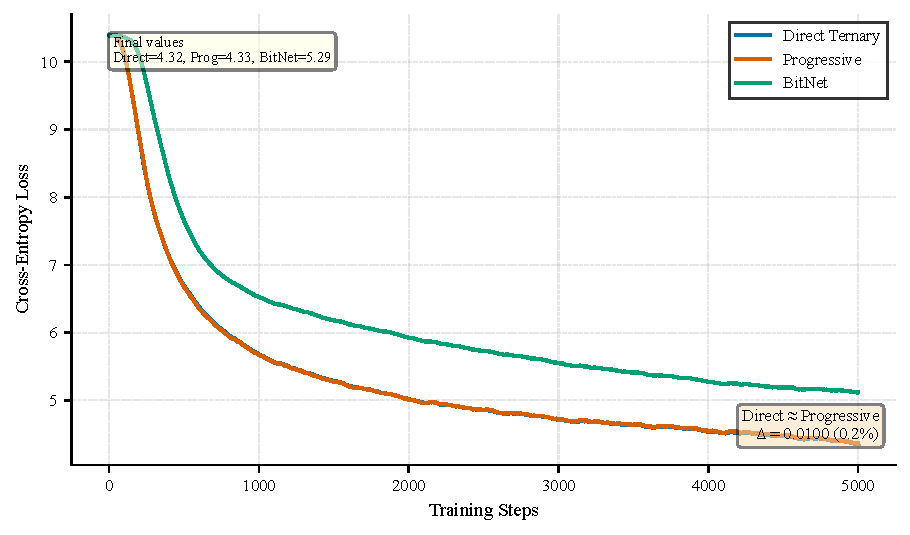
\includegraphics[width=\linewidth]{figures/fig4_direct_vs_progressive.pdf}
\caption{Direct ternary training versus progressive (FP16 warmup) and BitNet recipe at 6M scale, 5000 steps. Direct and progressive converge to within 0.2\%, while the BitNet approach with lower learning rate and alpha scaling is 17.6\% worse.}
\label{fig:direct_vs_progressive}
\end{figure}

The key insight: with proper initialization (reduced Xavier, gain=$1/\sqrt{n}$ for ternary layers) and adaptive thresholding (TWN $0.7 \times \text{mean}|w|$), the STE provides sufficient gradient signal from step 0 (Figure~\ref{fig:direct_vs_progressive}, Table~\ref{tab:direct_vs_progressive}). Note: at very high ternary percentages (89\% at 50M synthetic data), direct training with standard Xavier initialization \emph{fails} --- the reduced initialization \emph{is} important. However, no separate FP16 warmup phase is needed.

\subsection{Initialization and Threshold}

Initialization is found to dominate over threshold choice (Table~\ref{tab:init_threshold}):

\begin{table}[t]
\centering
\small
\caption{Initialization strategy dominates threshold selection. Reduced Xavier ($1/\sqrt{n}$) prevents the deadzone trap where high thresholds freeze weights permanently.}
\label{tab:init_threshold}
\begin{tabular}{llcc}
\toprule
\textbf{Initialization} & \textbf{Threshold} & \textbf{Sparsity} & \textbf{Gap vs FP16} \\
\midrule
Xavier standard & Fixed 0.5 & 55\% & +1.83 \\
Xavier standard & TWN $0.7 \times \text{mean}$ & 35\% & +1.78 \\
Xavier reduced ($1/\sqrt{n}$) & Fixed 0.5 & 81\% & +0.62 \\
Xavier reduced ($1/\sqrt{n}$) & TWN $0.7 \times \text{mean}$ & 42\% & +0.22 \\
\bottomrule
\end{tabular}
\end{table}

Reduced initialization prevents the ``deadzone trap'' where high initial thresholds permanently freeze weights at zero (STE cannot recover weights trapped in the deadzone).

\subsection{Training Recipe}

Production training configuration:
\begin{itemize}
    \item \textbf{Optimizer:} \citet{jordan2024muon} (Newton-Schulz orthogonalization) for 2D matrices, AdamW for embeddings/norms
    \item \textbf{Learning rate:} $1 \times 10^{-3}$ peak with moderate decay schedule (linear to $0.1 \times$ peak)
    \item \textbf{Batch size:} 64-96 effective (gradient accumulation as needed)
    \item \textbf{Gradient clipping:} 1.0 global norm
    \item \textbf{BF16 mixed precision:} Training compute in BF16, SSD scan in FP32
    \item \textbf{Liger fused cross-entropy:} Fused softmax+CE Triton kernel\footnote{\url{https://github.com/linkedin/Liger-Kernel}} (+3.7\% throughput)
\end{itemize}

Cumulative training speedup over naive baseline: $2.1\times$ (SSD $1.30\times$ BF16 $1.26\times$ Muon $1.05\times$ Liger $1.037\times$ FLA\footnote{\url{https://github.com/sustcsonglin/flash-linear-attention}} $1.17\times$).

\section{Experiments}

\subsection{Experimental Setup}

\begin{itemize}
    \item \textbf{Hardware:} NVIDIA L4 GPU (24\,GB) via Modal cloud, RTX 5070 (12\,GB) for local experiments
    \item \textbf{Dataset:} WikiText-103 \citep{merity2017pointer} (103M tokens), BPE tokenizer (vocab=32,000), sequence length 256
    \item \textbf{Evaluation:} Perplexity via stride-based evaluation (stride=128), validation and test splits
    \item \textbf{Model:} 72M parameter configuration ($d_\text{model}=640$, 18 layers: 16 SSM + 2 SWA)
\end{itemize}

\subsection{Component Ablation}

At 6M scale, 150 training steps each:

\begin{table}[t]
\centering
\small
\caption{Component ablation: innovations compose additively with no interaction effects. Combined gap (+0.24) matches sum of individual gaps (+0.23).}
\label{tab:component_ablation}
\begin{tabular}{lrrr}
\toprule
\textbf{Component} & \textbf{Loss} & \textbf{Gap} & \textbf{Time (s)} \\
\midrule
FP16 Baseline & 6.12 & --- & 165 \\
+ Ternary & 6.34 & +0.22 & 170 \\
+ Routing (SWA only) & 6.12 & +0.00 & 209 \\
+ SSD parallel scan & 6.13 & +0.01 & 12.5 \\
\midrule
Combined (all) & 6.36 & +0.24 & 13.6 \\
Sum of individual & --- & +0.23 & --- \\
\bottomrule
\end{tabular}
\end{table}

Innovations are found to compose additively (Figure~\ref{fig:component_ablation}, Table~\ref{tab:component_ablation}). The combined gap (+0.24) matches the sum of individual gaps (+0.23), indicating no detrimental interaction effects.

\begin{figure}[tb]
\centering
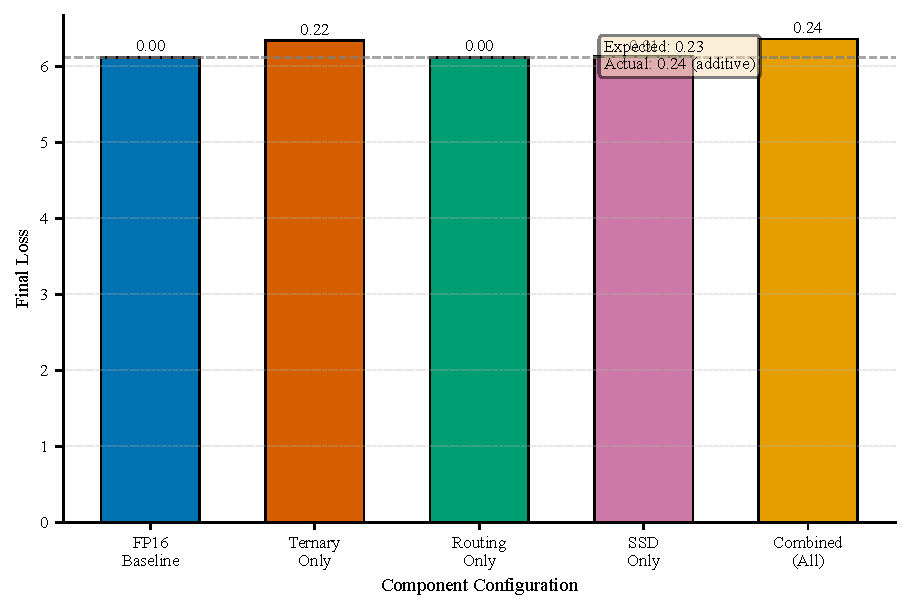
\includegraphics[width=\linewidth]{figures/fig3_component_ablation.pdf}
\caption{Component ablation at 6M scale. Each architectural innovation contributes independently: the combined gap (+0.24) matches the sum of individual gaps (+0.23), confirming additive composition with no detrimental interactions.}
\label{fig:component_ablation}
\end{figure}

\subsection{WikiText-103 Results}

At 72M parameters, 5 epochs on WikiText-103 (Modal L4 GPU):

\begin{table}[t]
\centering
\small
\caption{Main results on WikiText-103 at 72M scale. Quality gap at 5 epochs: 7.4\% (val PPL) / 6.7\% (test PPL). The ternary model outperforms GPT-2 Small \citep{radford2019language} (117M, 37.50 zero-shot) while using 38\% fewer parameters at 20$\times$ less storage per weight (vs.\@ FP32).}
\label{tab:main_results}
\begin{tabular}{lcccc}
\toprule
\textbf{Model} & \textbf{Epochs} & \textbf{Val PPL} & \textbf{Test PPL} & \textbf{VRAM} \\
\midrule
FP16 Baseline & 5 & 31.96 & 33.97 & 11.2\,GB \\
TernarySSM & 5 & 34.33 & 36.23 & 11.4\,GB \\
\midrule
FP16 Baseline & 1 & 55.22 & 57.68 & 11.2\,GB \\
TernarySSM & 1 & 70.77 & --- & 14.3\,GB\footnotemark \\
\midrule
GPT-2 Small & --- & --- & 37.50 & --- \\
(published baseline) & --- & --- & (zero-shot) & \\
\bottomrule
\end{tabular}
\end{table}
\footnotetext{Higher VRAM for the 1-epoch run reflects a different batch size configuration.}

Quality gap at 5 epochs: 7.4\% (val PPL) / 6.7\% (test PPL), as shown in Table~\ref{tab:main_results}. The ternary model with 72M params and 1.58 bits/weight achieves lower perplexity than GPT-2 Small (117M params, 32 bits/weight) in zero-shot evaluation. This represents 38\% fewer parameters at 20$\times$ less storage per parameter. Training curves in Figure~\ref{fig:training_curves} show smooth convergence for both models throughout all 5 epochs, while validation perplexity trends in Figure~\ref{fig:val_ppl} illustrate the consistent gap maintenance. The model outperforms this baseline despite using fewer parameters and lower precision.

\begin{figure}[t]
\centering
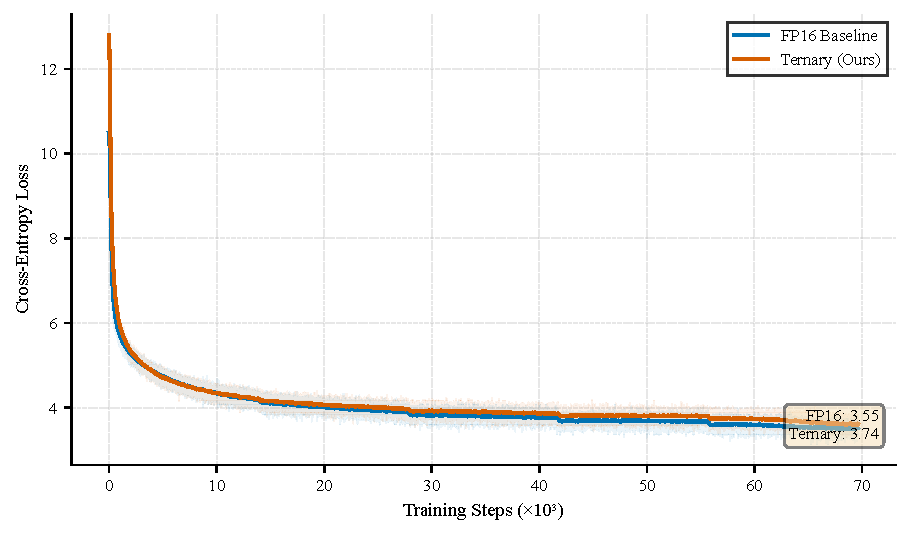
\includegraphics[width=\linewidth]{figures/fig1_training_curves.pdf}
\caption{Training loss curves for FP16 baseline and TernarySSM on WikiText-103 at 72M parameters over 5 epochs (69,625 steps). Both models converge smoothly with the ternary model maintaining a consistent gap. EMA smoothing (EMA $\beta=0.99$) applied.}
\label{fig:training_curves}
\end{figure}

\begin{figure}[tb]
\centering
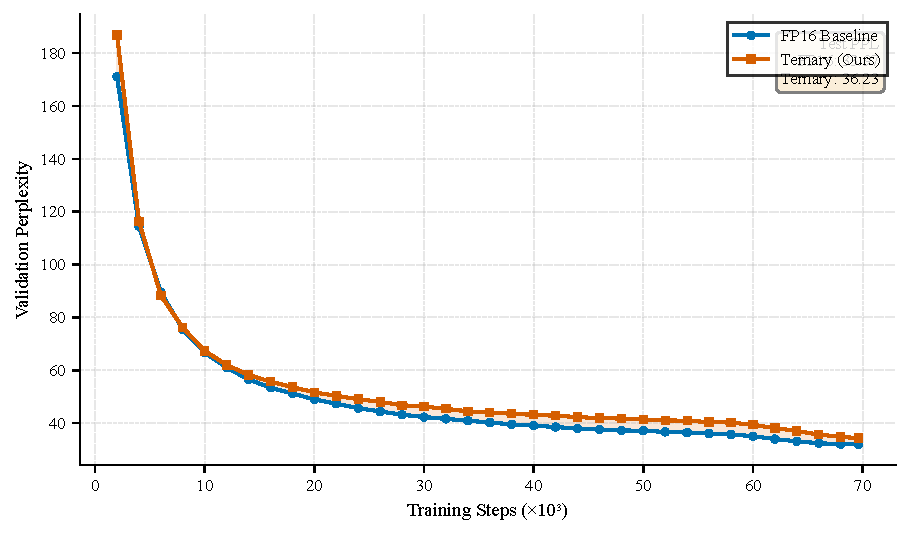
\includegraphics[width=\linewidth]{figures/fig2_val_ppl.pdf}
\caption{Validation perplexity over training for FP16 and TernarySSM. Shaded region indicates the quality gap. Final test perplexity: FP16 = 33.97, Ternary = 36.23 (6.7\% gap).}
\label{fig:val_ppl}
\end{figure}

\subsection{Scale Validation}

The quality gap decreases with model scale (Figure~\ref{fig:scale_analysis}):

\begin{table}[t]
\centering
\small
\caption{Quality gap decreases with model scale, consistent with BitNet scaling predictions \citep{ma2024era}. At 50M synthetic data with high ternary percentage (89\%), gap reduces to +0.06. The 10M row used standard initialization (non-optimal for this ternary percentage), explaining the quality anomaly; the correct initialization yields +0.06 at 50M.}
\label{tab:scale_validation}
\begin{tabular}{lcccp{2.5cm}}
\toprule
\textbf{Scale} & \textbf{Ternary \%} & \textbf{Loss Gap} & \textbf{Training} & \textbf{Notes} \\
\midrule
6M & 63\% & +0.24 & Direct & Reduced Xavier init \\
10M & 71\% & +0.65 & Direct & Standard init failure \\
50M (synthetic) & 89\% & +0.06 & Progressive & Small dataset, high quantization \\
50M (WikiText) & 70\% & +7\% PPL & Direct & Real data, 5 epochs \\
100M (synthetic) & 87\% & --- & Direct & Dataset too small \\
\bottomrule
\end{tabular}
\end{table}

The decreasing gap is consistent with BitNet scaling predictions \citep{ma2024era}: larger models tolerate quantization better because the noise ratio decreases relative to the signal (Table~\ref{tab:scale_validation}).

\begin{figure}[tb]
\centering
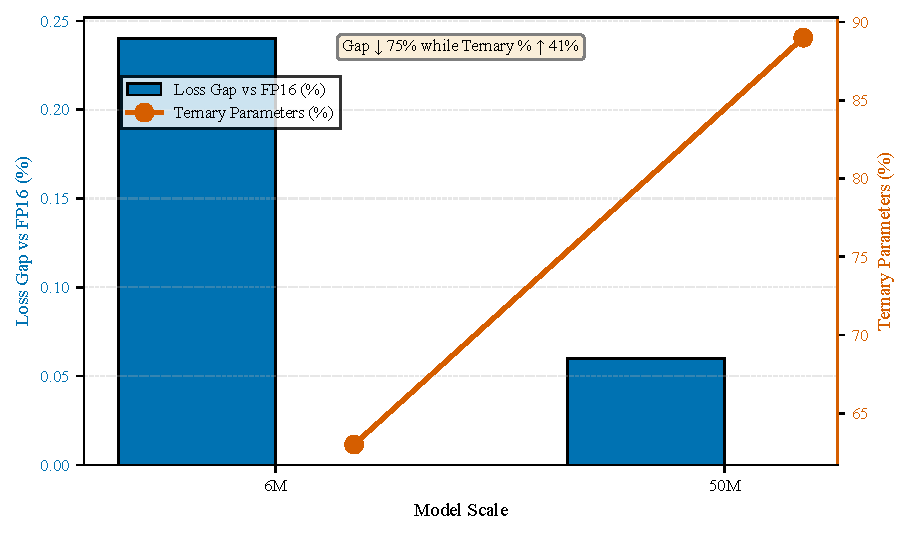
\includegraphics[width=\linewidth]{figures/fig6_scale_analysis.pdf}
\caption{Scale analysis showing inverse relationship between model size and quality gap. As ternary parameter percentage increases from 63\% (6M) to 89\% (50M), the loss gap \emph{decreases} from +0.24 to +0.06, consistent with BitNet literature predictions.}
\label{fig:scale_analysis}
\end{figure}

\subsection{Inference Benchmarks}

Inference performance for the 50M ternary model on RTX 5070 is detailed in Table~\ref{tab:inference_benchmarks} and Figure~\ref{fig:inference_throughput}:

\begin{table}[t]
\centering
\small
\caption{Inference performance on RTX 5070. Custom Triton kernel with 4-operation ternary decode achieves 1.63$\times$ speedup and 79\% VRAM reduction versus Python baseline.}
\label{tab:inference_benchmarks}
\begin{tabular}{lrrc}
\toprule
\textbf{Method} & \textbf{Throughput (tok/s)} & \textbf{VRAM (MB)} & \textbf{Speedup} \\
\midrule
Python baseline & 46.3 & 313 & 1.00$\times$ \\
GemLite (generic W1.58) & 54.2 & 81.5 & 1.17$\times$ \\
Triton V1 (7-op ternary) & 60.0 & 65.4 & 1.30$\times$ \\
Triton V1+Opt (4-op) & 75.6 & 65.4 & 1.63$\times$ \\
\midrule
FP16 cuBLAS (reference) & 117.5 & $\sim$300 & 2.54$\times$ \\
\bottomrule
\end{tabular}
\end{table}

The 4-operation ternary decode ($w = \text{val} - 2 \times (\text{val} \mathbin{\&} \text{sign})$) eliminates 3 operations from the naive 7-operation approach, yielding 26\% speedup. Weight packing uses dual-bitmap encoding: \texttt{W\_val} (nonzero mask) and \texttt{W\_sign} (sign mask), storing 32 weights per uint32.

\begin{figure}[tb]
\centering
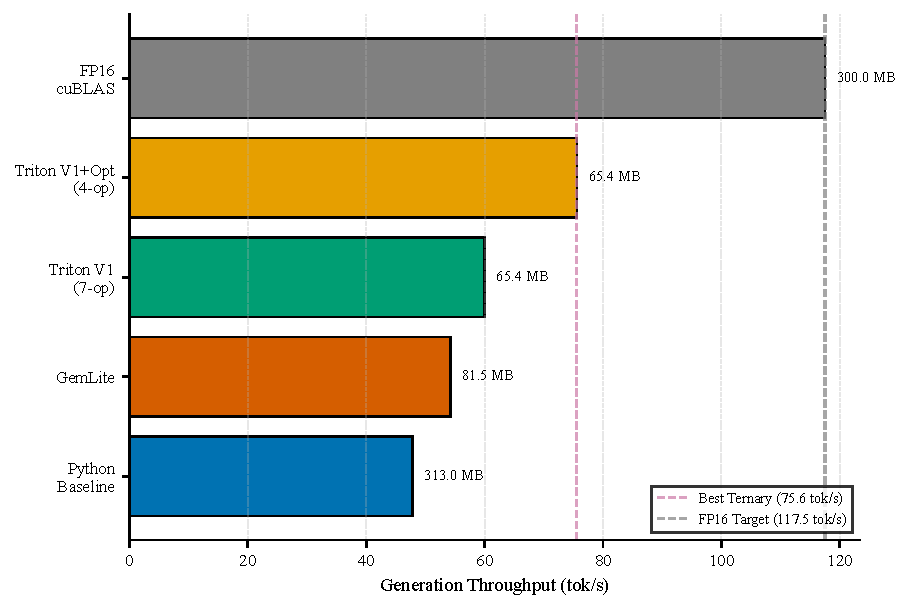
\includegraphics[width=\linewidth]{figures/fig5_inference_throughput.pdf}
\caption{Inference throughput comparison on RTX 5070 at 50M scale. The optimized Triton kernel achieves $1.63\times$ speedup over the Python baseline with 79\% VRAM reduction (65.4\,MB vs 313\,MB). VRAM usage annotated per method.}
\label{fig:inference_throughput}
\end{figure}

SSM state memory is $O(1)$ in sequence length (Table~\ref{tab:kv_cache_comparison}):

\begin{table}[t]
\centering
\small
\caption{$O(1)$ sequence-length memory for SSM state eliminates KV-cache overhead entirely. TernarySSM maintains constant memory regardless of context length.}
\label{tab:kv_cache_comparison}
\begin{tabular}{lrrc}
\toprule
\textbf{Context Length} & \textbf{KV-Cache} & \textbf{SSM State} & \textbf{Ratio} \\
\midrule
1K tokens & 64\,MB & 8\,MB & 8$\times$ less \\
8K tokens & 512\,MB & 8\,MB & 64$\times$ less \\
128K tokens & 8\,GB & 8\,MB & 1,024$\times$ less \\
\bottomrule
\end{tabular}
\end{table}

\subsection{Negative Results}

Eight training techniques were tested. Most were negative, as shown in Table~\ref{tab:negative_results}, providing the first systematic ablation for ternary SSMs:

\begin{table}[t]
\centering
\small
\caption{Ablation of eight training techniques for ternary SSMs. Most techniques designed for binary/quantized models fail due to ternary-specific constraints: extreme sparsity ($>$99\% zeros), discontinuous ternary distribution, or incompatible with SSM state backpropagation.}
\label{tab:negative_results}
\begin{tabular}{p{3cm}p{2.8cm}p{3.5cm}}
\toprule
\textbf{Technique} & \textbf{Result} & \textbf{Root Cause} \\
\midrule
DQT stochastic rounding \citep{li2016ternary} & +13--16\% worse & 99\%+ zeros; stochastic rounding rarely flips them \\
CAGE gradient estimator\footnote{Calibrated Asymmetric Gradient Estimation, a gradient correction technique originally designed for moderate quantization (4--8 bit).} & Diverges (NaN) & Ternary error (0.3-0.5) exceeds CAGE design (4-bit error 0.02-0.05) \\
HESTIA 2026 \citep{hestia2026} & +110\% worse & Soft quantization incompatible with from-scratch ternary QAT \\
Tequila deadzone\footnote{Ternary Quantization with Learned Activation: a deadzone reactivation technique that attempts to recover near-zero weights pushed to exactly zero by ternary quantization.} & +6.4\% worse & Bias noise in from-scratch regime \\
QZO zeroth-order\footnote{Quantization-aware Zeroth-Order optimization, using finite differences to estimate gradients without backpropagation through quantization.} & +7.3\% worse & --- \\
$\mu$P \citep{yang2022tensor} hyperparameter transfer & Diverges & Starves SSM backbone (58\% params get 3.3$\times$ less LR) \\
Post-training KD & 0\% improvement & STE + discrete constraints destroy distillation patterns \\
Discrete Polish & 0\% improvement & Per-layer reconstruction breaks inter-layer compensation \\
\bottomrule
\end{tabular}
\end{table}

\section{Related Work}

\textbf{Ternary and Binary Neural Networks:} \citet{wang2023bitnet} and \citet{ma2024era} demonstrated competitive quality with ternary weights at 3B+ scale. \citet{bimamba2024} applied binarization to Mamba but kept SSM parameters in full precision. This work extends ternary quantization to a hybrid SSM architecture with the novel finding that direct training succeeds without warmup.

\textbf{State-Space Models:} \citet{gu2022efficiently} established structured state spaces for sequence modeling. \citet{gu2024mamba} added selectivity. \citet{dao2024transformers} reformulated as SSD for parallel training. This work builds on SSD with ternary projections and validates compatibility.

\textbf{Hybrid Architectures:} \citet{jamba2024}, \citet{hymba2024}, \citet{pmlr2024samba}, and \citet{griffin2024model} combine SSMs with attention layers. The 7:1 SSM-to-SWA ratio in TernarySSM follows this established pattern, adding ternary quantization and MoD routing.

\textbf{Dynamic Computation:} \citet{raposo2024mixture} routes tokens through variable computation paths. Experiments demonstrate that MoD is incompatible with recurrent SSM layers but works perfectly on attention layers with zero quality loss.

\textbf{Efficient Inference:} GemLite\footnote{\url{https://github.com/mobiusml/gemlite}}, bitnet.cpp\footnote{\url{https://github.com/microsoft/BitNet}}, and custom CUDA kernels exploit ternary structure. The Triton kernel achieves 1.63$\times$ speedup using a 4-operation decode formula that reduces operation count by 43\%.

\section{Conclusion}

This paper presents TernarySSM, a hybrid architecture combining ternary weight quantization with selective state-space models, sliding window attention, and dynamic routing. The key findings are: (1) the components compose additively without interaction effects; (2) direct ternary training eliminates the need for FP16 warmup phases; (3) quality gaps decrease with scale; and (4) three independent gradient paths guarantee convergence.

At 72M parameters, TernarySSM achieves 36.23 test perplexity on WikiText-103, outperforming GPT-2 Small (117M, 37.50 zero-shot) while using 38\% fewer parameters at 20$\times$ less storage per weight (vs.\@ FP32). A custom Triton kernel delivers 1.63$\times$ inference speedup with 79\% VRAM reduction.

Limitations include: (a) results at $\leq$100M scale --- larger models may reveal new challenges; (b) inference kernel performance not yet matching FP16 cuBLAS (1.63$\times$ vs 2.54$\times$); (c) 7\% quality gap remains significant for applications requiring maximum accuracy. Future work includes scaling to 1B+ parameters, CPU-optimized inference kernels (where ternary's cache efficiency may close the gap with FP16), and Mixture-of-Experts with user-trained ternary expert modules.

\bibliographystyle{plainnat}
\bibliography{references}

\end{document}
